\chapter{Conclusion}
\label{chapter6}

%\setlength{\epigraphrule}{0pt}
\epigraph{\textit{If you can't fly then run, if you can't run then walk, if you can't walk then crawl, but whatever you do you have to keep moving forward.}}{ -- Martin Luther King Jr.}

% **************************** Define Graphics Path **************************
\ifpdf
    \graphicspath{{Chapter6/Figs/Raster/}{Chapter6/Figs/PDF/}{Chapter6/Figs/}}
\else
    \graphicspath{{Chapter6/Figs/Vector/}{Chapter6/Figs/}}
\fi

\section{Summary}

Recognizing complex event in videos has become an important task in computer vision due to various applications. However, this is a challenging task because we have to deal with real videos. In summary, there are four main challenges that we need to handle:
\begin{enumerate}
	\itemsep0em 
	\item \textit{Large content variation}.
	\item \textit{Uncontrolled capturing condition.}
	\item \textit{Large scale video dataset.}	
	\item \textit{Near-miss videos.}
\end{enumerate}
	
  The most important challenge that need to be handled is \textit{uncontrolled capturing condition}. This challenge of internet videos often harm the performance of event detection systems that was built on action recognition techniques. We handle this challenge by decomposing the original videos into segments and investigating \textit{feature representation}, \textit{feature aggregation}, and \textit{feature learning} methods from these segments. Beside this main challenge, we also deal with the \textit{large content variation} and \textit{large scale video dataset} as well. To this end, we made following contributions (Fig. \ref{c6_contribution}):

\begin{figure}
	\centering
	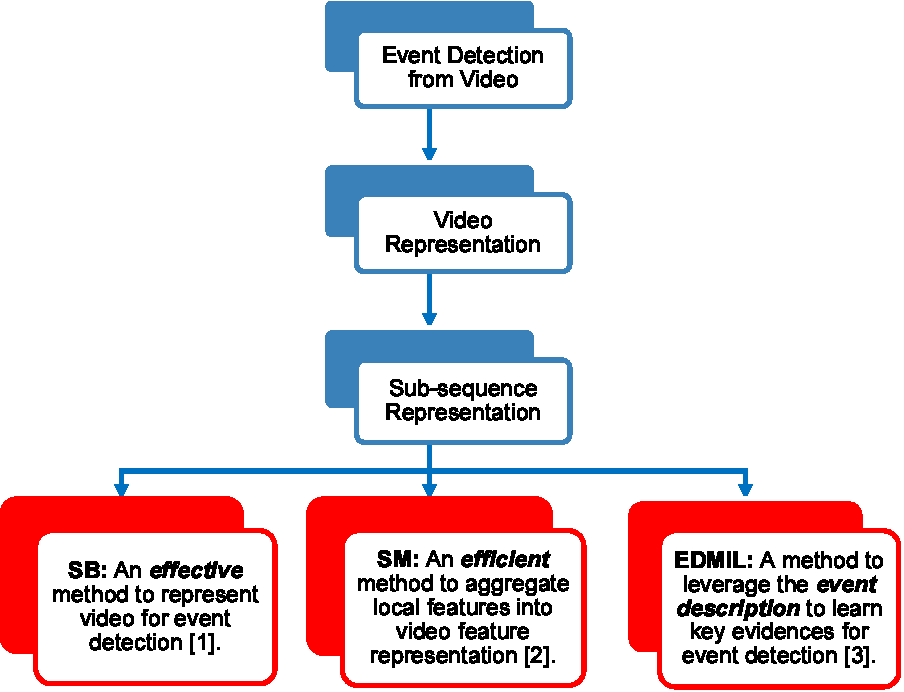
\includegraphics[width=1\textwidth]{contribution.pdf}
	\caption{Summary of contributions of my dissertation.}
	\label{c6_contribution}
\end{figure}

\begin{enumerate}
	\item We propose a new \textit{feature representation} method, named segment-based representation (\textbf{SB}), to overcome the limitations of the traditional video-based approaches. The basic idea is to examine shorter segments instead of using the representative frames or entire video. We carry thorough experiments to verify our proposed method by investigating different strategies to decompose a video into segments. These strategies include uniform segment sampling and segments based on shot boundary detection. By using more training examples (at segment level), this method can handle the \textit{large content variation} challenge as well.
	
	\item We propose a new \textit{feature aggregation} method, called sum-max video pooling (\textbf{SM}), to deal with noisy information in complex videos. This pooling technique is based on the layer structure of video. Basically, we apply sum pooling at the low layer representation while using max pooling at the high layer representation. Sum pooling is used to keep sufficient relevant features at the low layer, while max pooling is used to retrieve the most relevant features at the high layer, therefore it can discard irrelevant features in the final video representation. Our video pooling method is very efficient, thus it can be applied to \textit{large scale video dataset} as well.
	
	\item We propose a new \textit{feature learning} method, named Event-driven Multiple Instance Learning (\textbf{EDMIL}), to learn key evidences for complex event detection. We treat each segment as an instance and model it in a multiple instance learning framework \cite{andrews2002support}, where each video is a ``bag''. The instance-event similarity is quantized into different levels of relatedness. Intuitively, the most (ir)relevant instances should have higher (dis)similarities. Therefore, we propose to learn the instance labels by jointly optimizing the instance classifier and its related level. Similar to the first contribution, this method also use more training examples (at segment level), therefore it can handle the \textit{large content variation} challenge.
\end{enumerate}

It is beneficial to use some engineering tricks in order to handle large scale dataset. For example, the pre-computed kernel is suitable when there is a large number of events. In this case, we only need to calculate the kernel one time and train multiple time with different labels. This technique is especially useful in our EDMIL method.

A summary of the significant achievement of our proposed methods can be seen in Fig. \ref{c6_summary}. Our methods (SB, SM and EDMIL) can improve the baseline VideoBOW by \textbf{22.55\%}, \textbf{2.67\%} and \textbf{43.62\%} respectively on the large scale MED 2011 dataset.

\begin{figure}
	\centering
	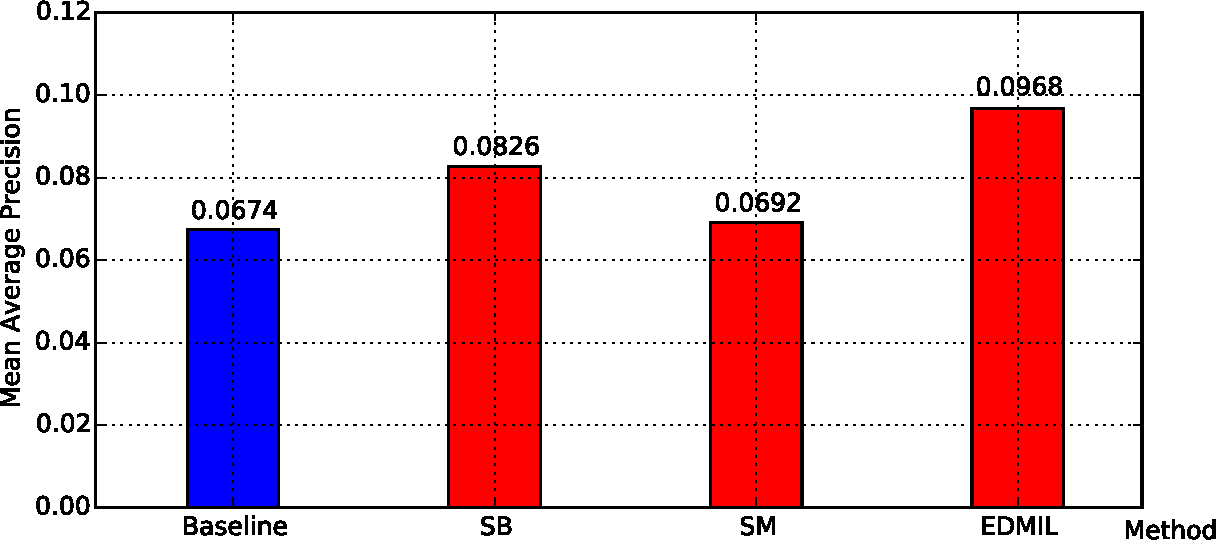
\includegraphics[width=1\textwidth]{summary.pdf}
	\caption{Performance comparison of our proposed solutions on the large scale MED 2011 dataset.}
	\label{c6_summary}
\end{figure}
	
\section{Conclusion}	
	Detecting event in video is a challenging yet worth pursuing research topic. Due to nature of internet videos, which often contains irrelevant content, it is crucial to develop robust technologies for event detection in realistic videos. This dissertation has addressed this challenging issue by introducing three major techniques including a feature representation, feature aggregation and feature learning method.
	
	At first, we proposed using the segment-based approach for event detection. Our proposed segment-based approach outperforms the video-based approach in most cases when using a simple non-overlapping sampling strategy. More interestingly, the results are significantly improved when we using the segment-based approach with an overlapping sampling strategy.  This suggests the importance of segment localization on the event detection performance. Suppose the segment length is fixed, we are interested in determining which segment is the best representative for an event. In this study, we also observed that the detection performance is quite sensitive to the segment-length and it depends on the dataset. The results obtained from the late fusion strategy is quite stable and close the peak performance. This suggests a methodical way to generalize the segment-based approach to other datasets. However, this method is not scalable because it requires a lot of computation costs. Therefore, learning an optimal segment length for each event can be beneficial for an event detection system.
	
	Secondly, we proposed to use a sum-max video pooling technique to combine both sum pooling and max pooling into a holistic video representation. This pooling technique is based on the layered structure of video. Preliminary results showed that this is an promising direction for video representation. One limitation of the current approach is that the performance depends on the segment length. Therefore, we suggest to investigate a better approach to utilize the layered structure of video for video representation.
	
	Lastly, we proposed a new feature learning method to detect event in videos from its key evidences. Our method differs from others in that we utilize the evidential description provided for each event. Given this supportive information, we search for key evidences by jointly optimizing with instance feature in a variant of multiple instance learning framework. As a result, we obtained a superior event detection performance.
	
\section{Future Work}
We plan to extend our work in following directions.
\begin{itemize}
	\item \textbf{Learning the relationship between segments}. Currently, we can learn a set of important segments that can be used for event detection. We have not imposed any constraints on the relation between segments. However, some spatial-temporal relationship might be important to identify an event. For example, in the event ``changing a vehicle tire'', the action ``removing hubcap'' should take place before the action ``replacing tire''. Or in the event ``flash mob gathering'', the ``gathering'' action should happen before the ``dancing'' action takes place. Moreover, some actions can have a co-occurrence relationship. For example, in the ``birthday party'' event, people can be both singing and dancing. 
	\item \textbf{Learning the importance of each concept in the concept bank} for event detection. Currently we only detect a set of concepts that can be used to provide evidences to detect an event. These concepts are obtained from NLP techniques. However, we do not know if it really visually represents for that event. It is interesting know which concepts that both textually and visually represent for an event.
	\item \textbf{Video description generation}. This is the task that describing about what happening in a video. This task also has many practical applications such as helping blind or visually impaired people understand what happening in videos. Besides, it can be used to build question-answering systems, which provides an interactive mechanism for a better understanding of the video. Moreover, this technology, as a result, can be applied to zero-shot event detection, as illustrated in Fig. \ref{c6_zeroshot}.
	
	\begin{figure}
		\centering
		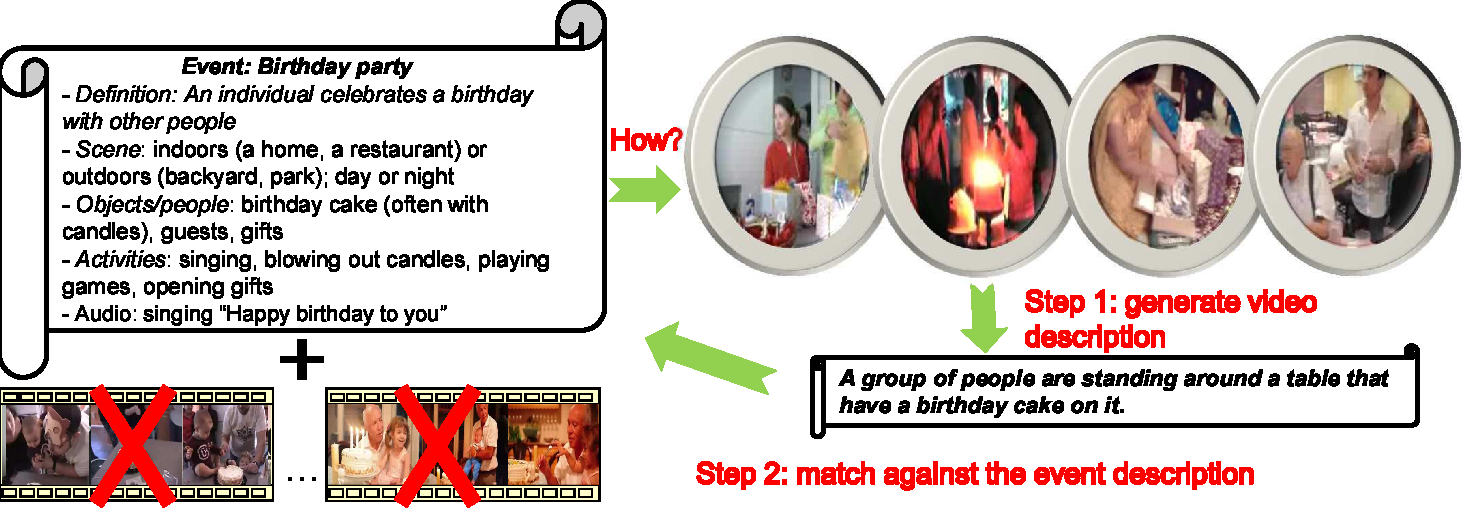
\includegraphics[width=1\textwidth]{zeroshot.pdf}
		\caption{Illustration of video event description and video event detection.}
		\label{c6_zeroshot}
	\end{figure}
\end{itemize}
